\documentclass[12pt,a4paper]{report}
\usepackage[a4paper,left=1in,right=1in,top=1in,bottom=1in]{geometry}

\usepackage{listings}
\usepackage{color}
 
\definecolor{codegreen}{rgb}{0,0.6,0}
\definecolor{codegray}{rgb}{0.5,0.5,0.5}
\definecolor{codepurple}{rgb}{0.58,0,0.82}
 
\lstdefinestyle{mystyle}{ 
    commentstyle=\color{codegreen},
    keywordstyle=\color{magenta},
    numberstyle=\tiny\color{codegray},
    stringstyle=\color{codepurple},
    basicstyle=\normalfont\ttfamily,
    breakatwhitespace=false,         
    breaklines=true,                 
    captionpos=b,                    
    keepspaces=true,                 
    numbers=left,                    
    numbersep=5pt,                  
    showspaces=false,                
    showstringspaces=false,
    showtabs=false,                  
    tabsize=3
}
 
\lstset{style=mystyle}

\usepackage{amssymb}
\usepackage{booktabs}
\usepackage{setspace}
\usepackage{tabularx}
\usepackage[pdftex]{graphicx} %for embedding images
\usepackage{url} %for proper url entries
\usepackage[bookmarks, colorlinks=false, pdfborder={0 0 0}, pdftitle={Quad-Pi Report}, pdfauthor={Tushaar G.}, pdfsubject={Minor Project Report}, pdfkeywords={RPi, Parallel, Emotion, OpenCV}]{hyperref} %for creating links in the pdf version and other additional pdf attributes, no effect on the printed document
\usepackage[final]{pdfpages} %for embedding another pdf, remove if not required

% Drawing block diagrams
\usepackage{tikz}
\usetikzlibrary{positioning,fit,calc}
\tikzset{block/.style={draw,thick,text width=3cm,minimum height=1.5cm,align=center},
         line/.style={-latex}
}

% Drawing Gantt charts
\usepackage{pgfgantt}

% Justifying tables
\usepackage{array}

% Plots
\usepackage{pgfplots}
\pgfplotsset{width=16cm,compat=1.5}

% Algorithm
\usepackage[ruled, vlined, linesnumbered]{algorithm2e}
\usepackage{setspace}

%Page Border
\usepackage{pgf}
\usepackage{pgfpages}

\pgfpagesdeclarelayout{boxed}
{
  \edef\pgfpageoptionborder{0pt}
}
{
  \pgfpagesphysicalpageoptions
  {%
    logical pages=1,%
  }
  \pgfpageslogicalpageoptions{1}
  {
    border code=\pgfsetlinewidth{1pt}\pgfstroke,%
    border shrink=\pgfpageoptionborder,%
    resized width=.88\pgfphysicalwidth,%
    resized height=.88\pgfphysicalheight,%
    center=\pgfpoint{.5\pgfphysicalwidth}{.5\pgfphysicalheight}%
  }%
}
\pgfpagesuselayout{boxed}
\setlength{\parindent}{1cm}

\begin{document}
\linespread{1.3}
\renewcommand\bibname{References} %Renames "Bibliography" to "References" on ref page

%include other pages
\pagenumbering{gobble}
\begin{titlepage}

\begin{center}
\vspace{2mm}
\textup{\small \textit{Project Report On}}\\

% Title
\Large \textbf {ToViS: Topic Based Video Suggestion System}\\[0.5in]

% Submitted by
\normalsize \textit{Submitted by} \\
\begin{table}[h]
\centering
\bgroup
\def\arraystretch{1.4}
\begin{tabular}{lcr}
\textbf{15IT117} & & \textbf{Tushaar Gangarapu} \\
\textbf{15IT119} & & \textbf{Himadri Pal} \\ 
\textbf{15IT130} & & \textbf{Pratyush Prakash} \\
\textbf{15IT146} & & \textbf{Suraj Hegde} \\
\end{tabular}
\egroup
\end{table}

\textbf{VI Semester B.Tech (IT)}\\[0.4in]

\textit{Under the guidance of}\\\vspace{3mm}
{\textbf{Dr. Sowmya Kamath S}}\\
{\textbf{Department of IT, NITK Surathkal}}\\[0.4in]

       \small \emph{in partial fulfillment for the award of the degree\\\vspace{2mm} of}
        \vspace{.3in}

       {\bf Bachelor of Technology} \\\vspace{2mm} \textit{in} \\\vspace{2mm} {\bf Information Technology} \\\vspace{2mm} \textit{at}\\[0.3in]

% Bottom of the page

\includegraphics[width=0.2\textwidth]{images/logo}\\
\Large{Department of Information Technology}\\
\normalsize
\textsc{National Institute of Technology Karnataka, Surathkal}\\
March 2018 \\
\vspace{0.3cm}

\end{center}

\end{titlepage}

\newpage
\thispagestyle{empty}

\begin{center}

\huge{Department of Information Technology}\\[0.5cm]
\normalsize
\textsc{National Institute of Technology Karnataka, Surathkal}\\[2.0cm]

\emph{\LARGE Certificate}\\[2cm]
\end{center}
\normalsize This is to certify that this is a bonafide record of the project entitled ``\textbf{ToViS: Topic Based Video Suggestion System}'' presented by the students whose names are given below during VI semester 2018 in partial fulfilment of the requirements of the degree of Bachelor of Technology in Information Technology.\\[1.0cm]

\begin{table}[h]
\centering
\bgroup
\def\arraystretch{1.2}
\begin{tabular}{lcr}
Register No. & & Name of Student \\ \\ \hline
\\
15IT117 & & Tushaar Gangarapu \\ 
15IT119 & & Himadri Pal \\
15IT130 & & Pratyush Prakash \\
15IT146 & & Suraj Hegde \\
\end{tabular}
\egroup
\end{table}

\vfill


% Bottom of the page
\noindent
\begin{tabular}[t]{@{}l} 
\\
Date: \today
\end{tabular}
\hfill% move it to the right
\begin{tabular}[t]{r@{}}
Dr. Sowmya Kamath S \\
(Project Guide)
\end{tabular}

\newpage
\thispagestyle{empty}

\begin{center}

\huge{Department of Information Technology}\\[0.5cm]
\normalsize
\textsc{National Institute of Technology Karnataka, Surathkal}\\[2.0cm]

\emph{\LARGE Declaration}\\[2cm]
\end{center}
\normalsize We hereby declare that the Project Work Report entitled ``\textbf{ToViS: Topic Based Video Suggestion System}'' which is being submitted to {\bf National Institute of Technology Karnataka, Surathkal} in accordance with the completion of the minor project for the degree of {\bf Bachelor of Technology} in {\bf Information Technology} is a bonafide report of the work carried out by us. \\[1.0cm]

\begin{table}[h]
\centering
\bgroup
\def\arraystretch{1.2}
\begin{tabular}{lcr}
Register No. & & Name of Student \\ \\ \hline
\\
15IT117 & & Tushaar Gangarapu \\ 
15IT119 & & Himadri Pal \\
15IT130 & & Pratyush Prakash \\
15IT146 & & Suraj Hegde \\
\end{tabular}
\egroup
\end{table}

\vfill


% Bottom of the page
\begin{flushleft}
Department of Information Technology \\
Place: NITK, Surathkal \\
Date: \today
\end{flushleft}



\includepdf[pages=27-]{references/similarity.pdf}

\cleardoublepage
%\pagebreak
\phantomsection
\addcontentsline{toc}{chapter}{Acknowledgements}
\chapter*{Acknowledgments}
We would like to express our appreciation to all those who have helped us in the successful completion of this project, directly and indirectly. \par
Firstly, we would like to express our sincere gratitude to our guide \textit{Dr. Sowmya Kamath S}, Department of Information Technology, NITK Surathkal for her insightful advice and guidance throughout the course of our project work. Without her continued support and interest, this project would not have been the same as presented here.\par
This project would have been impossible without the help of our hostel mates, who took their valuable time to provide inputs to our model development process. Also, we express our thanks to all the teaching and non-teaching staff in the Department of Information Technology for their invaluable support.

\vfill

% Bottom of the page
\noindent
\begin{tabular}[t]{@{}l} 
\\
\\
\today \\
{National Institute of Technology Karnataka}\
\end{tabular}
\hfill% move it to the right
\begin{tabular}[t]{r@{}}
Tushaar Gangarapu \\
Himadri Pal \\
Pratyush Prakash \\
Suraj Hegde
\end{tabular}
\vspace{2in}
\begin{abstract}

The exponential growth of web content over the last couple of years has been a promoter and boost for advances in movie recommendation and retrieval. This report focuses on the methodology used for suggesting similar movies to the user based on the view they are currently watching. Collaborative filtering has been the predominant and the current state of the art technique for recommendation of movies. In this report, we show that using a topicality measure for grouping related movies outperforms the collaborative filtering model which uses suffers from the low sparsity and presentation and position bias. Our model also performs better in terms of tackling popularity bias. The topicality based recommendation uses a combination of two approaches to rank the movies. The first approach involves using the applying the traditional inverse document frequency (\textit{idf}) heuristic to the movies. The second approach takes into account user feedback in the form of co view information and various heuristics defined in the methodology are applied. The experiment is conducted on the \textit{IMDb dataset}. In addition, we show that employing user feedback improves user rating and engagement when compared with the collaborative filtering approach. 


\end{abstract} 


\pagenumbering{roman} %numbering before main content starts
\tableofcontents
\listoffigures
\listoftables

\newpage
\pagenumbering{arabic} %reset numbering to normal for the main content

\chapter{Introduction}

In the past few years, the video content on the Internet increased tremendously. Advancements in social media (Facebook, Twitter, Instagram etc.) have resulted in an abundance of content supply and demand. It has been observed that the number of people willing to spend more time on a website are relatively very less. Now-a-days related video recommendation is \textit{ubiquitous} and \textit{pervasive} on the Internet. From YouTube statistics it can be inferred that over six billion hours of movies have been watched every month. Furthermore, video upload rate is 100 movies per minute. All the above mentioned reasons led to the necessity of development of sophisticated technology for movie retrieval, discovery and recommendations. Movie suggestions are the movies the user is presented with, in relevance to the current movie being watched ($V_W$).\par
The movies being recommended can be purely content based (tags, genres etc.) or can be collaborative filtering based (used by most of the modern recommender systems). Recommendations via collaborative filtering approach is suitable for movies with good views while the same fails for fresh content and tail videos which have very noisy and sparse co-view data. To overcome sparsity and noise related issues, researchers have combined collaborative filtering with content based models to develop hybrid models. CNN, Netflix, Hulu etc. all use hybrid recommender systems to improve \textit{user's browsing experience} through click-through analytics and co-view data.\par
Usually movie (video) is modeled as a set of content data which includes a set of \textit{data topics} extracted from many sources such as metadata, Wikipedia articles, uploader keywords (frequently used), freebase entities, common queries used to search, names of play-lists. Then, these assigned (weighted) topics are used to obtain a set of related movies (videos) for recommendations and suggestions. Furthermore, to achieve an \textit{effective topic based} movie representation, weights are assigned to each topic tagged with a movie. Two techniques have been presented to associate weights to topics. The first technique involves a well known retrieval method which uses  inverse document frequencies (\textit{idf}) and topic frequencies (\textit{tf}). The second technique involves using the implicit (explicit) user feedback. Now, this feedback can be utilized to learn the optimal weights of topics (supervised learning).\par
The topic based representation of the movie being watched ($V_W$) is a \textit{query} which is addressed to the inverted index, the index saves video representations based on topics as \textit{documents}. This way, the movie suggestion problem can be seen as a \textit{retrieval of movies-over-inverted index of documents}. To find the most optimal movie recommendations (even in large volumes of videos), usage of query optimization algorithms can improve efficiency. The top ranked videos (documents) retrieved as a result to the query ($V_W$) are suggested to the viewer as a set of \textbf{content based} video recommendations which (recommendations) can either be presented to the user without any modifications or are appended to the results of co-view based movie (video) recommender (hybrid modeling) system.

\chapter{Literature Review}

\section{Background}

There has been immense progress in the field of video retrieval due to the increasing user base and user demands on video sharing sites like YouTube, dailymotion, etc. This has led to addressing the various drawbacks and challenges to this video recommendation system. 

One of the common challenges includes the position bias which is the case with most retrieval systems. Position bias is the positive bias which is introduced towards the first few retrieved results. Sometimes users even neglect the last couple of videos retrieved by the IR system. This leads to those videos getting a bad feedback recursively and finally the system starts ignoring them. Hence both the system and user relevance is affected. \par
However it was seen that position bias is not the only bias affecting the system. Yisong Yue et. al \cite{yue2010} introduced a new concept of presentation bias. This sort of bias is predominantly seen in all on-line video sharing platforms. Presentation bias is introduced when the one set of videos have title bolding and the other set doesn’t. This prompts the user to select the video from the former set even though their quality is low or they are not related. Title Bolded videos are perceived by the users to be more attractive.\par
The existing video recommendation systems heavily rely on collaborative filtering as a method to suggest videos. These systems are based on co-view data. Both Davidson et. al. \cite{davison2010} and Baluja et. al. \cite{baluja2008} describe such a system. The reason for the success of co view based filtering is because the metadata could be noisy. This is seen in the case when user closes the browser before the system receives the long-watch notification. So, there is inconsistency in the various metrics like abandonment rate. Whereas co-view graphs are nothing but directed graphs depicting a particular user session. Baluja et. al. \cite{baluja2008} introduces a concept of an adsorption algorithm. It’s a learning and classification framework which uses a rich graph structure and labelled objects.\par
Collaborative filtering as a method performs well for popular and frequently watched videos but in the case of fresher and tail content videos there is a massive degradation in performance. The reason for this is that the co-view data is noisy and sparse. Hence this filtering algorithm would not be effective if it’s only based on co-view data.\par
To tackle this some hybrid approaches have been experimented and implemented. Bo Yang \cite{yang2007} presents a hybrid approach based on relevance feedback and multi-modal fusion. Their model is capable of working without any user preference information. This is very different from the traditional approaches. The multi-modal relevance is depicted by aural, video and textual relevance which is used to recommend videos. However their system was only tested for a small portion of TRECVID dataset having preset sample videos. Hence the system would not be favorable for a large collection of videos.\par
The approach given below is a hybrid approach tested for a larger audience and a large movie database. Table \ref{tab:1} summarizes the existing works.

\begin{table}[h]
  \centering
  \bgroup
  \def\arraystretch{1.5}
  \caption{Summary of Existing Works}
  \label{tab:1}
  \begin{tabular}{>{\raggedright}p{2.4cm}>{\raggedright}p{3cm}>{\raggedright}p{4cm}>{\raggedright}p{4cm}} 
    \toprule
    \textbf{Author} & \textbf{Approach} & \textbf{Merits} & \textbf{Limitations} \tabularnewline
    \midrule
     Davidson J. et al. \cite{davison2010} & Collaborative filtering & Recommendations are more accurate & Presentation bias, only co-viewed videos 
 \tabularnewline
     Shumeet Baluja et al. \cite{baluja2008} & Co-view graph & Recommendations are more accurate & Presentation bias, only co-viewed videos \tabularnewline
     Bo Yang et al. \cite{yang2007} & Hybrid model & Considers both video info and co-views (multimodal) & Small scale \tabularnewline
    \bottomrule
  \end{tabular}
  \egroup
\end{table}

\section{Identified Gaps}
This session briefs about the gaps in the existing recommender systems based on the literature survey. Firstly, the existing recommender (suggestion) systems base their existence on \textit{collaborative filtering} methods, which might work for popular, more viewed, more liked, dense data; while the same fails for sparse data and tail (fresh) videos. It can also be seen that there is a lack of \textit{content based} video retrieval systems. Also, \textit{topic based retrieval} has never been done on a large scale.

\section{Problem Statement}
Given a large corpus of movies (here, movie trailers) and appropriate metadata (genre and user submitted tags); propose  a methodology to suggest a list of movies the user would like to watch next based on the current movie.

\section{Objectives}

The main objective of the recommendation system is to suggest to the user what she would enjoy watching next based on the current movie. This is done by representing user feedback in the form of a co-view based graph. In the representation of this co-view based graph, every movie is represented by a \textit{node}. The current node is linked to any other nodes, if they are often watched in the same session. The nodes in the proximity of the query node and related to the topic is suggested to the user. To find the topical relation,a hybrid dataset composed of the \textit{IMDb movie dataset} comprising of last 35 years of movies and their respective genres along with a set of user defined tags is used. 
\chapter{Methodology}

\section{Experimental Setup for Data Collection}

To form the co-view graph, \textbf{twenty} people had been chosen (not randomly to not induce bias), and their preferences were noted. The students selected were of varied departments including both circuit and non-circuit branches of different age and linguistic groups with varied tastes and preferences. This was done so as to eliminate any bias that might be introduced as a result of ``similar'' set of people. They were given a start movie and asked to navigate through to 10 other movies. They however were not asked to watch the movies due to their length, but instead movie \textit{trailers} were used. In this manner, a list of \textbf{ten} co-viewed movies was obtained for each movie as the start movie. There were a total of \textbf{five} sessions per participant that spanned at different times (not immediately) for over a month. The participants were also asked to tag the watched movies/trailers (user defined tags).

\section{Tagging the Dataset}
To tag the movies, a database of user submitted tags was collected. The movie tags are a combination of the set of genres of a movie and the user submitted tags. These tags were ultimately appended along with the coviews to a common csv file \texttt{coview\_movie.csv}.

\section{Topical Analysis}
\subsection{Topic Count Computation}

Next, the topic count function was implemented. The topic count function for a particular movie, $V_W$ and a given topic $\tau$ returns the number of movies in the co-view graph having the same topic as the target movie. Here the random unrelated movies which might be seen by the user get a count ($c(\cdot)$ in equation \ref{eq:1}) value of \textbf{zero} hence they get a score value of zero. Hence, they are omitted.

\subsection{Inverse Document Frequency (\textit{idf}) of Topics}

We apply the traditional information retrieval heuristic -- inverse document frequency (\textit{idf}) on the topics. This is calculated for all the topics. This is a normalization technique which ensures that rare topics get equal priority as the common ones. This list is stored as a dictionary and the computation is \textit{done only once} so that the prediction-time overheads decrease. This component is attributed by $log(1 + df(\cdot))$ in equation \ref{eq:1}, where $df(\cdot)$ is the document frequency.

\subsection{Quality Factor and Stop Words}

Since the topic terms obtained from the user submitted tags and the genres \textit{do not} contain any stop-words, we need not explicitly normalize the terms during indexing and querying. So, the factor that indicates stop word removal ($\mathcal{I}_s(\cdot)$) is considered to be \textbf{one} (equation \ref{eq:1}). We assume the Quality of the video ($q(\cdot)$) to be \textbf{one} (equation \ref{eq:1}). The quality factor is based on factors like ``thumbs up'', ``thumbs down'', video popularity etc. But since these factors introduce a popularity bias, these are not added. 

\begin{equation}
\label{eq:1}
	sc(V_W, V_R) = q(V_R) \sum \limits_{\tau \in V_W \cap V_R} \mathcal{I}_s(\tau) \cdot \frac{c(\tau, V_W)}{log(1 + df(\tau))} \cdot c(\tau, V_R)
\end{equation}

\section{Scoring}

Our final function is the \textit{scoring function} derived from equation \ref{eq:1} is defined as in equation \ref{eq:2}.

\begin{equation}
\label{eq:2}
	sc(V_W, V_R) = \sum \limits_{\tau \in V_W \cap V_R} \frac{c(\tau, V_W)}{log(1 + df(\tau))} \cdot c(\tau, V_R)
\end{equation}

This function computes the similarity score ($sc(V_W, V_R)$) between two videos $V_W$ , $V_R$. This similarity measure is calculated for all the videos compared with the current video or movie being watched. These similarity scores are then sorted in order and the videos corresponding to top \textbf{ten} similarity scores are presented to the user as watch movie recommendations. \par 
We define a \textit{session}, to be the time until which the user chooses one of the videos recommended to the user by the system. The session starts with the user getting a random video or movie (during experiment) or the user selecting some movie. Then the above scores are generated and the videos are presented. The user can accordingly select the next movie or choose to end the session. 

\section{ToViS: The Video Suggestion Model}

\textbf{ToViS} is a video suggestion system that basically is a hybrid model. The model mainly focuses on topic based movie retrieval (see section 3.1 for experimental setup) combined with collaborative filtering methods to obtain near optimal recommendations. The block diagram representing the same is depicted as in Figure \ref{block}. Topic retrieval and Topic indexing are the main areas of focus in this research.

\begin{figure}
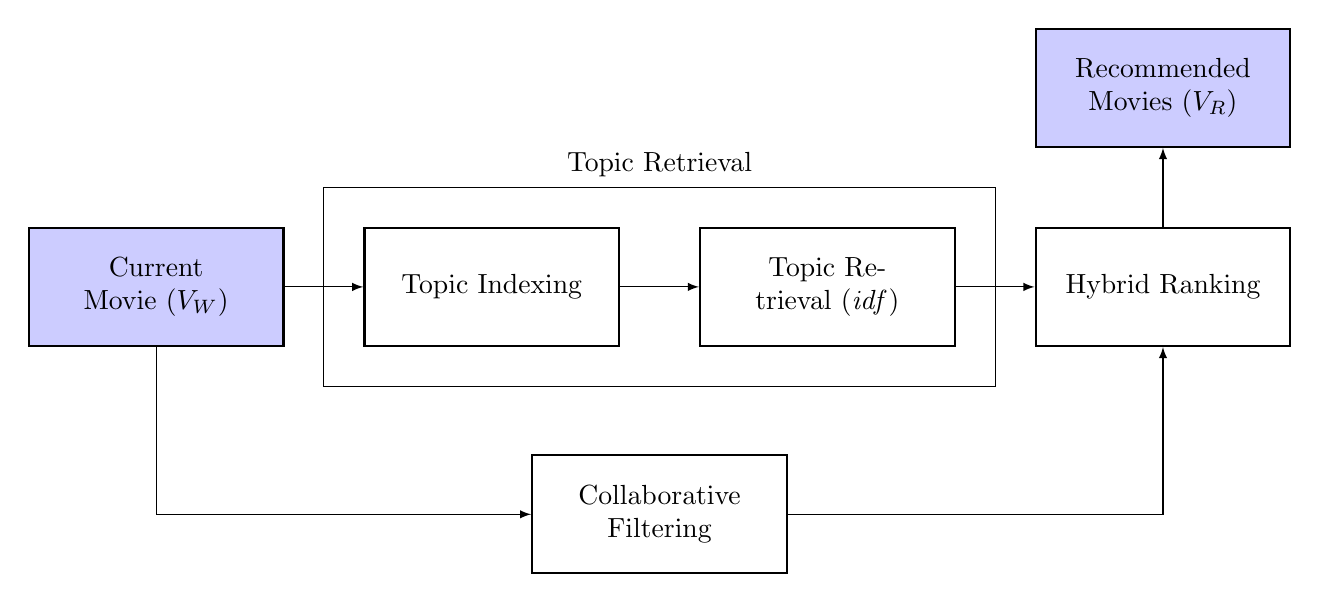
\begin{tikzpicture}
  \node[block,fill=blue!20] (a) {Current Movie ($V_W$)};
  \node[block,right=of a] (b) {Topic Indexing};
  \node[block,right=of b] (c) {Topic Retrieval (\textit{idf})};
  \node[block,right=of c] (d) {Hybrid Ranking};
  \node[block,above=of d,fill=blue!20] (f) {Recommended Movies ($V_R$)};
  \node[draw,inner xsep=5mm,inner ysep=5mm,fit=(b)(c),label={90:Topic Retrieval}]{};
  \draw[line] (a)-- (b);
  \draw[line] (b) -- node[name=u] {$$} (c);
  \draw[line] (c) -- (d);
  \node[block,below=2cm of u] (e) {Collaborative Filtering};
  \draw[line] (a) |- (e);
  \draw[line] (e) -| (d);
  \draw[line] (d) -- (f);
\end{tikzpicture}
\caption{\textit{ToViS} Process Model Diagram}
\label{block}
\end{figure}

\chapter{Implementation}

\section{Work Done}
The system built uses two retrieval techniques, suggestions based on topical and collaborative filtering. The users were given the liberty to select the first movie. Based on the above described methodology the co-view graph was used to calculate the score of all the other movies with respect to the current movie. The top ten movies were ranked and suggested to the user. \par
Our work incorporated both the user feedback and topic based on inverted index. This allowed our model to be robust. The user feedback also made room for unrelated movie recommendations. This was because the during the process of collecting co views users tend to deviate from the genres and teleport to some random genre. Hence those changes were visible in the co-view graph.

\section{Results and Analysis}

The following section describes the evaluation methodology, metrics used and the evaluation outcomes. We have used, user-centered evaluation metrics -- watch time, completion rate, abandonment rate.

\subsection{Evaluation Methodology}
There are many ways of evaluating systems like the one presented here (ToViS) -- online studies, user studies and historical data based user simulation. We must note that the sample test subjects chosen must represent the population subjects as much as possible. This is necessary to avoid any bias in decision and perception resulting from personal judgments. In addition to selecting the `perfect sample', explicit feedback collection from the selected users might result in intrusion and irritation.\par
If a user is to evaluate the given system would result in varied opinions based on a lot of `bias' factors -- culture, emotion, location etc. Table \ref{tab:2} represents the \textbf{Likert Evaluation} of the proposed system with respect to the experimental setup (section 3.1). The following section presents a much more apt evaluation methodology.

\begin{table}[h]
  \centering
  \bgroup
  \def\arraystretch{1.5}
  \caption{Summary of Likert Evaluation (20 users)}
  \label{tab:2}
  \begin{tabular}{>{\raggedright}p{4.5cm}>{\raggedright}p{1.8cm}>{\raggedright}p{1.8cm}>{\raggedright}p{1.8cm}>{\raggedright}p{1.9cm}>{\raggedright}p{1.9cm}} 
    \toprule
    \textbf{Question Asked} & \textbf{Strongly Agree} & \textbf{Agree} & \textbf{Neutral} & \textbf{Disagree} & \textbf{Strongly Disagree} \tabularnewline
    \midrule
     Did the recommender system recommend relevant videos? & 3 & 8 & 6 & 1
& 2 \tabularnewline
     Did your session time increase as result of suggestions? & 1 & 3 & 10 & 4 & 2 \tabularnewline
     Did you have Overall Satisfaction? & 4 & 6 & 7 & 2 & 1 \tabularnewline
    \bottomrule
  \end{tabular}
  \egroup
\end{table}

\subsection{Evaluation Metrics and Evaluation}

We have used much more apt evaluation metrics that were user centered. \textbf{Watch time} is the total time a user spends watching videos (movies) on ToViS. \textbf{Completion rate} is the number of videos that were presented to the user by ToViS and were watched completely. \textit{Abandonment rate} is the number of movies (videos) that the user watches up-until the point where the user \textit{does not} continue the session (watch any of the recommendations). \par
The evaluation of the system with the above mentioned metrics has been carried out in the experimental setup (section 3.1). Watch time (see Figure \ref{res:1}), Completion rate (see Figure \ref{res:2}) and Abandonment rate (see Figure \ref{res:3}) were captured for all 20 users and then these were averaged for overall evaluation (see Figure \ref{res:4}). Figures \ref{res:5} to \ref{res:8} represent the User Interface for ToViS. 

\begin{figure}
	\centering
	\label{res:1}
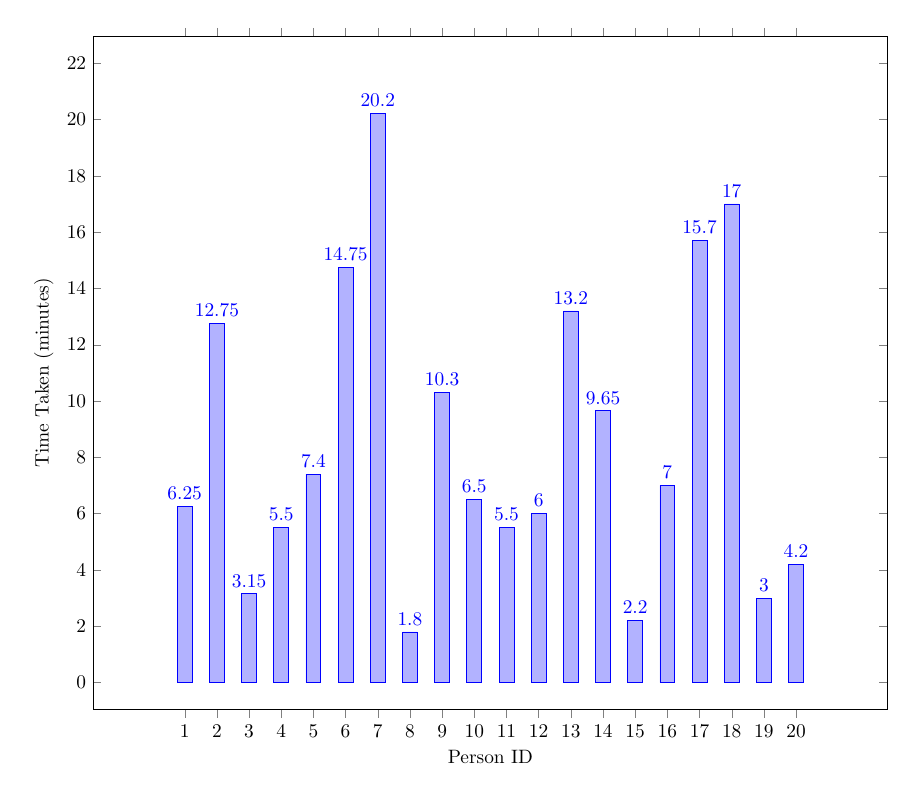
\begin{tikzpicture}[scale=0.7]
	\begin{axis}[
	    ybar,
        bar width=0.27cm,
    	enlargelimits=0.15,
    	legend style={at={(0.5,-0.15)},
      	anchor=north,legend columns=-1},
        xlabel={Person ID},
    	ylabel={Time Taken (minutes)},
    	symbolic x coords={1, 2, 3, 4, 5, 6, 7, 8, 9, 10, 11, 12, 13, 14, 15, 16, 17, 18, 19, 20},
    	xtick=data,
    	nodes near coords,
    	nodes near coords align={vertical},
    ]
	\addplot coordinates {(1, 6.25) (2, 12.75) (3, 3.15) (4, 5.50) (5, 7.40) (6, 14.75) (7, 20.20) (8, 1.80) (9, 10.30) (10, 6.5) (11, 5.5) (12, 6) (13, 13.20) (14, 9.65) (15, 2.2) (16, 7) (17, 15.70) (18, 17) (19, 3) (20, 4.2)};
    \end{axis}
\end{tikzpicture}
	\caption{Watch Time for 20 Users (Based on Experimental Setup)}
\end{figure}


\begin{figure}
	\centering
	\label{res:2}
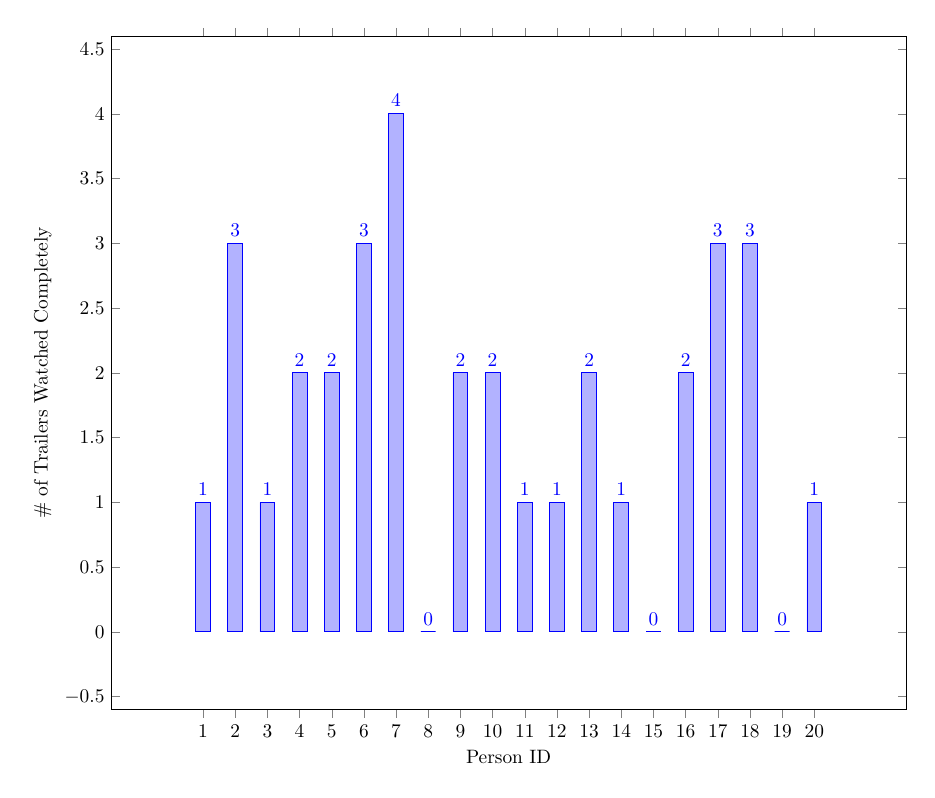
\begin{tikzpicture}[scale=0.7]
	\begin{axis}[
	    ybar,
        bar width=0.27cm,
    	enlargelimits=0.15,
    	legend style={at={(0.5,-0.15)},
      	anchor=north,legend columns=-1},
        xlabel={Person ID},
    	ylabel={\# of Trailers Watched Completely},
    	symbolic x coords={1, 2, 3, 4, 5, 6, 7, 8, 9, 10, 11, 12, 13, 14, 15, 16, 17, 18, 19, 20},
    	xtick=data,
    	nodes near coords,
    	nodes near coords align={vertical},
    ]
	\addplot coordinates {(1, 1) (2, 3) (3, 1) (4, 2) (5, 2) (6, 3) (7, 4) (8, 0) (9, 2) (10, 2) (11, 1) (12, 1) (13, 2) (14, 1) (15, 0) (16, 2) (17, 3) (18, 3) (19, 0) (20, 1)};
    \end{axis}
\end{tikzpicture}
	\caption{Completion Rate for 20 Users (Based on Experimental Setup)}
\end{figure}

\begin{figure}
	\centering
	\label{res:3}
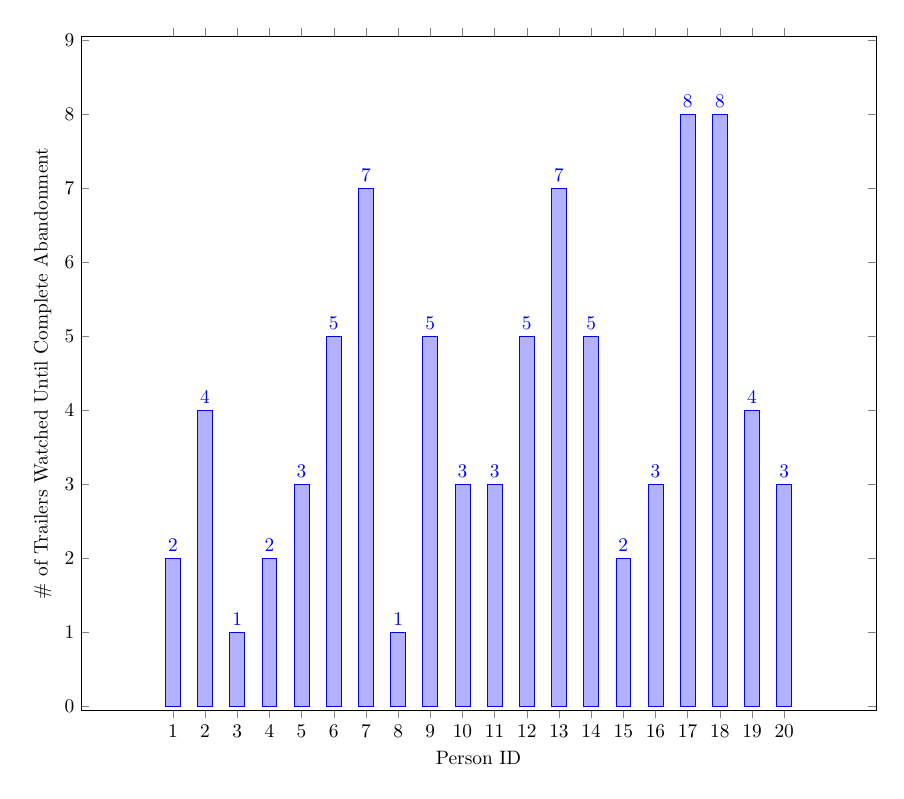
\begin{tikzpicture}[scale=0.7]
	\begin{axis}[
	    ybar,
        bar width=0.27cm,
    	enlargelimits=0.15,
    	legend style={at={(0.5,-0.15)},
      	anchor=north,legend columns=-1},
        xlabel={Person ID},
    	ylabel={\# of Trailers Watched Until Complete Abandonment},
    	symbolic x coords={1, 2, 3, 4, 5, 6, 7, 8, 9, 10, 11, 12, 13, 14, 15, 16, 17, 18, 19, 20},
    	xtick=data,
    	nodes near coords,
    	nodes near coords align={vertical},
    ]
	\addplot coordinates {(1, 2) (2, 4) (3, 1) (4, 2) (5, 3) (6, 5) (7, 7) (8, 1) (9, 5) (10, 3) (11, 3) (12, 5) (13, 7) (14, 5) (15, 2) (16, 3) (17, 8) (18, 8) (19, 4) (20, 3)};
    \end{axis}
\end{tikzpicture}
	\caption{Completion Rate for 20 Users (Based on Experimental Setup)}
\end{figure}

\begin{figure}
	\centering
	\label{res:4}
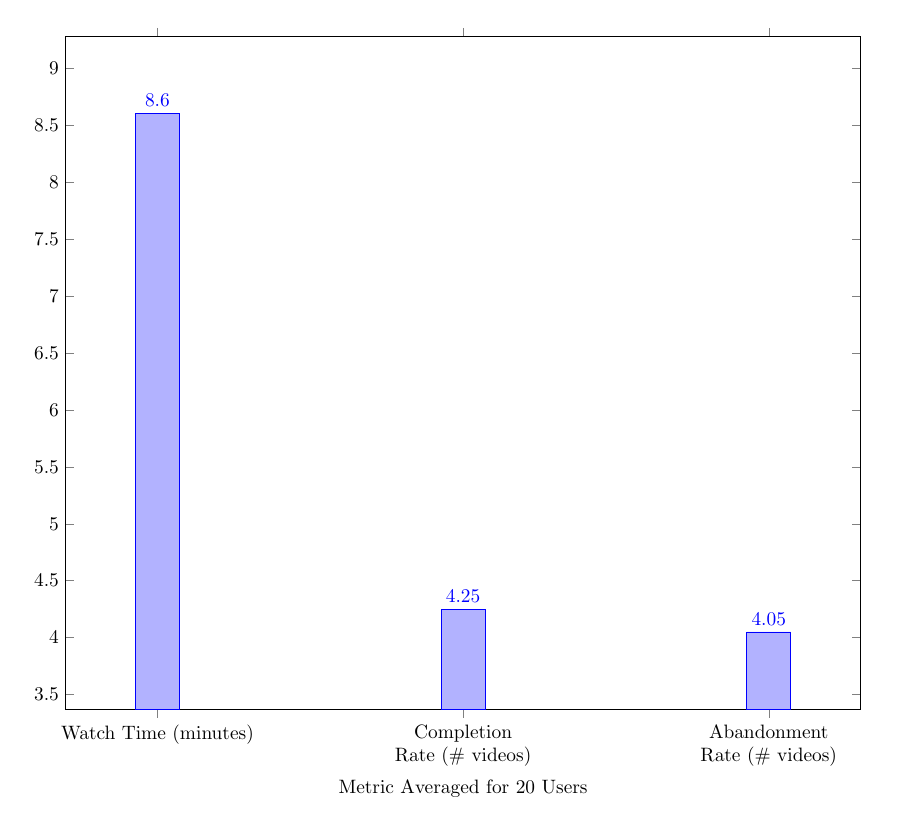
\begin{tikzpicture}[scale=0.7]
	\begin{axis}[
	    ybar,
        x tick label style={text width=4cm, align=center},
        bar width=0.8cm,
    	enlargelimits=0.15,
    	legend style={at={(0.5,-0.15)},
      	anchor=north,legend columns=-1},
        xlabel={Metric Averaged for 20 Users},
    	symbolic x coords={Watch Time (minutes), Completion Rate (\# videos), Abandonment Rate (\# videos)},
    	xtick=data,
    	nodes near coords,
    	nodes near coords align={vertical},
    ]
	\addplot coordinates {(Watch Time (minutes), 8.6025) (Completion Rate (\# videos), 4.25) (Abandonment Rate (\# videos), 4.05)};
    \end{axis}
\end{tikzpicture}
	\caption{Averaged Evaluation Metrics Used for User Relevance Evaluation}
\end{figure}

\begin{figure}[htb]
\centering

\includegraphics[scale=0.35]{images/img1}
\caption{User Interface for ToViS (I)}
\label{res:5}
\end{figure}

\begin{figure}[htb]
\centering

\includegraphics[scale=0.35]{images/img2}
\caption{User Interface for ToViS (II)}
\label{res:6}
\end{figure}

\begin{figure}[htb]
\centering
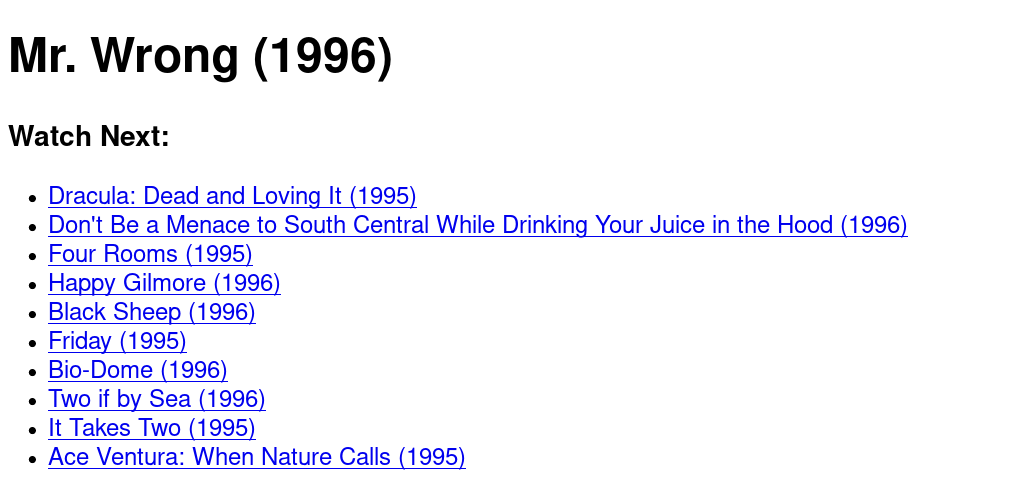
\includegraphics[scale=0.35]{images/img3}
\caption{User Interface for ToViS (III)}
\label{res:7}
\end{figure}

\begin{figure}[htb]
\centering
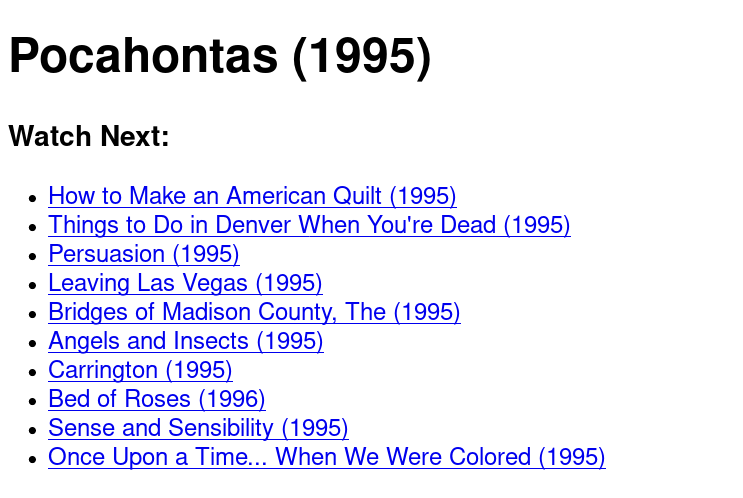
\includegraphics[scale=0.35]{images/img4}
\caption{User Interface for ToViS (IV)}
\label{res:8}
\end{figure}


\section{Innovative Work}

We added a novel concept of building the co-view graph by approaching a wide range of users and constructing a feedback loop. These metrics formed the basis for our model which was later coupled with the topic based recommendations.

\section{Details of each individual's work w.r.t. project tasks}

The individual contributions and the project time-line has been progressively represented in the form of a Gantt chart as in Figure \ref{contr:1}.

\begin{figure}[htb]
\centering
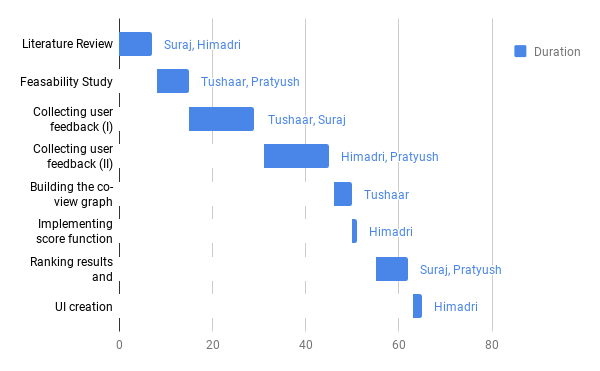
\includegraphics[scale=0.7]{images/chart}
\caption{Gantt Chart Representing the Work Flow and Individual Contributions}
\label{contr:1}
\end{figure}
\chapter{Conclusion and Future Work}

In our work, we address the challenges faced by the current most famous model of collaborative filtering. While considering popular and regularly watched videos the user based filtering model gives an accurate recommendation. However for fresh and tail content videos, the collaborative model fails horribly. Our model takes into account the topics of individual videos. Hence this problem is tackled. User engagement increases by using our model of user feedback. \par
Topicality based retrieval also outperforms collaborative filtering in terms of avoiding the various biases which affect the retrieval system in the form of noise. The hybrid model expressed in the last section would include the best of both worlds.\par
As the size of the movie database increases it wouldn’t be possible to perform computation for the entire database especially in the case of multiple clients. Hence some optimization techniques like WeakAnd needs to be implemented which would consider only a subset of the dataset. This random sample collected from the dataset should accurately describe the dataset. WeakAnd query optimization scores a subset of the entire document so that it crosses a given threshold. \par
The performance of the model can be further improved by merging it with the collaborative filtering model. However, in this case there would be a need to rerank all the results obtained from both the topic based model and the collaborative model. This reranking function should not be biased towards any one model. Hence the parameters used must either be common for both the models and must have equal weightage in the models or must not overlap with any of the models. The latter one is prefered as it introduces a new metric which might further improve the recall and precision. This hybrid model could outperform both the models.\par
Dynamic updation of the topic weights could make our model an evolutionary one. Given enough time, our model would keep improving and performing better.
\cleardoublepage
%\pagebreak
\phantomsection
\addcontentsline{toc}{chapter}{References}
\begin{thebibliography}{99}

\bibitem{michael2014}Bendersky, Michael, et al. (2014). ``Up next: retrieval methods for large scale related video suggestion.'' Proceedings of the 20th ACM SIGKDD international conference on Knowledge discovery and data mining, ACM.

\bibitem{yue2010}Yue, Yisong, Rajan Patel, and Hein Roehrig. (2010). ``Beyond position bias: Examining result attractiveness as a source of presentation bias in clickthrough data.'' Proceedings of the 19th international conference on World wide web, ACM.

\bibitem{davison2010}Davidson, James, et al. (2010). ``The YouTube video recommendation system.'' Proceedings of the fourth ACM conference on Recommender systems, ACM.

\bibitem{baluja2008}Baluja, Shumeet, et al. (2008). ``Video suggestion and discovery for youtube: taking random walks through the view graph.'' Proceedings of the 17th international conference on World Wide Web, ACM.

\bibitem{yang2007}Yang, Bo, et al. (2007). ``Online video recommendation based on multimodal fusion and relevance feedback.'' Proceedings of the 6th ACM international conference on Image and video retrieval, ACM.

\end{thebibliography}

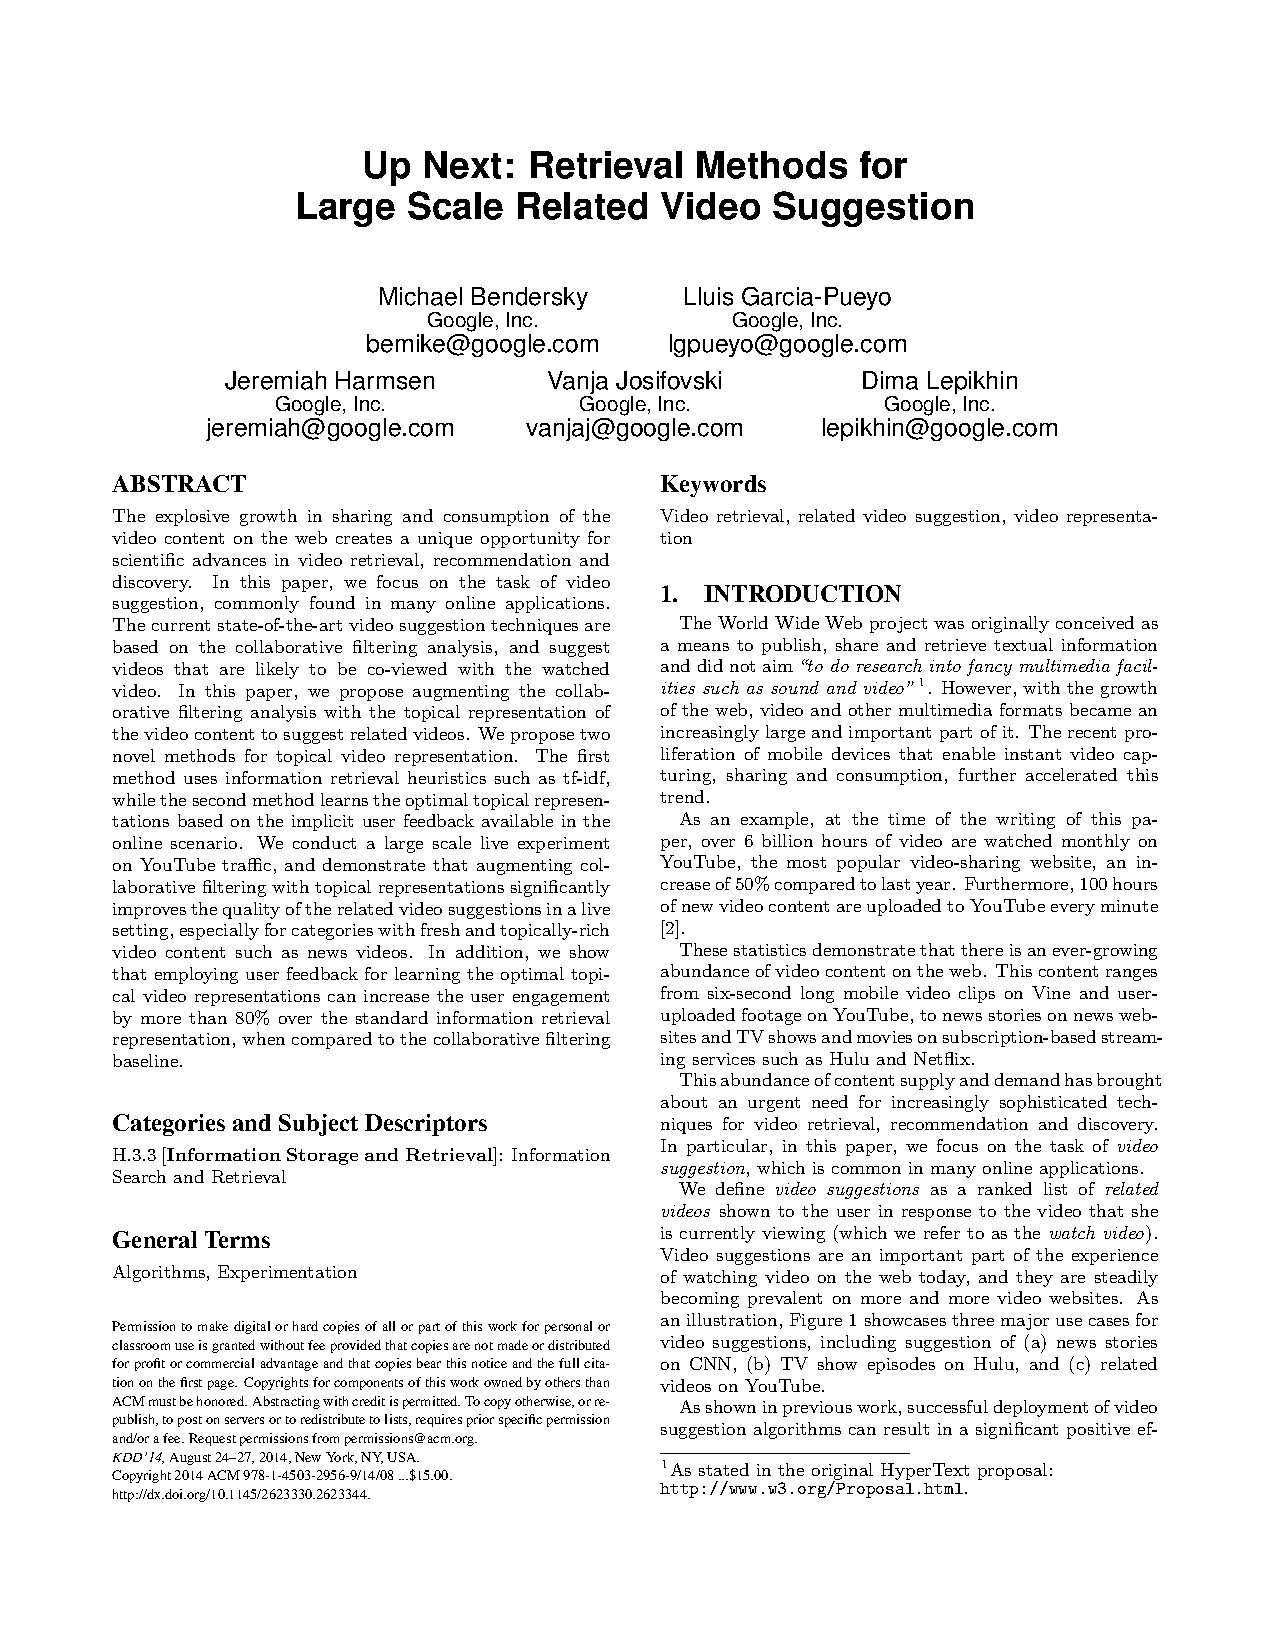
\includepdf[pages=-]{references/UpNext.pdf}

\end{document}
